\documentclass[aip,amsmath,amssymb,reprint, jcp]{revtex4-1}
\usepackage{tikz}
\usepackage{graphicx}% Include figure files
\usepackage{dcolumn}% Align table columns on decimal point
\usepackage{bm}% bold math
%My packages start
%\usepackage{subfig}
\usepackage{multirow}					
\usepackage{array}
%\usepackage{booktabs}
\usepackage{footnote} 
\newcommand{\angstrom}{\text{\normalfont\AA}}
\usepackage{booktabs}
\usepackage{float}
\usepackage{mathtools}
\usepackage{color}
\usepackage{natmove}
\newcommand{\comment}[1]{\noindent \textcolor{blue}{#1}}

% Extra packages (MP):

\usepackage{tikz}
\usetikzlibrary{shapes,arrows,decorations.markings}

\newcommand*{\citen}[1]{%
  \begingroup
    \romannumeral-`\x % remove space at the beginning of \setcitestyle
    \setcitestyle{numbers}%
    \cite{#1}%
  \endgroup   
}

\begin{document}

\title[]{Water induced Restructuring of Vanadia clusters supported on a-TiO$_2$ (101) hydration dynamics}
%\author{Kræn Christoffer}
%\author{Siva Chiriki}
%\author{B.\ Hammer}
%\email{hammer@phys.au.dk}
%\affiliation{ 
%Department of Physics and Astronomy, Aarhus University, DK-8000 Aarhus C, Denmark.
%}
% \homepage{phys.au.dk}
 
\date{\today}% It is always \today, today,
             %  but any date may be explicitly specified

\begin{abstract}

\end{abstract}
\maketitle

% Introduction
\section{\label{sec:introduction}Introduction}
\section{Experimental Claim}
After the deposition of vanadium oxide clusters on clean anatase-TiO$_2$ (101) surface, they exposed to water. In the same experiment they de-exposed the water and captured the STM images at all instances of partial water vapour pressure 
(P${_\text{O}{_2}}$) conditions. The final STM images ware shown in Fig. 1 (a), vanadium oxide clusters on clean surface, Fig 1(b)- vanadium oxide clusters after reaction with water and Fig. 1(c)- vanadium oxide clusters when they de-expose  water after the reaction happens.   

In Fig 1(a), only one feature observed and in Fig 1(b) and 1(c) there are two distinct features ware observed. The observations  from STM images from Fig 1(a) - Fig 1(b), indicates that there is restructuring of these vanadium clusters due to reaction between water and vanadium oxide clusters. The STM image (Fig 1(c)) during de-exposure,  indicating that there is reshaping of vanadium oxide clusters after reaction with water. And interestingly they achieved the reversibility between Fig 1(c) to Fig 1(b) and vice-versa. This gives an evidence that due to water reaction with vanadium oxide clusters, they were not observed same features as on clean surface.         

\begin{figure*}[h]
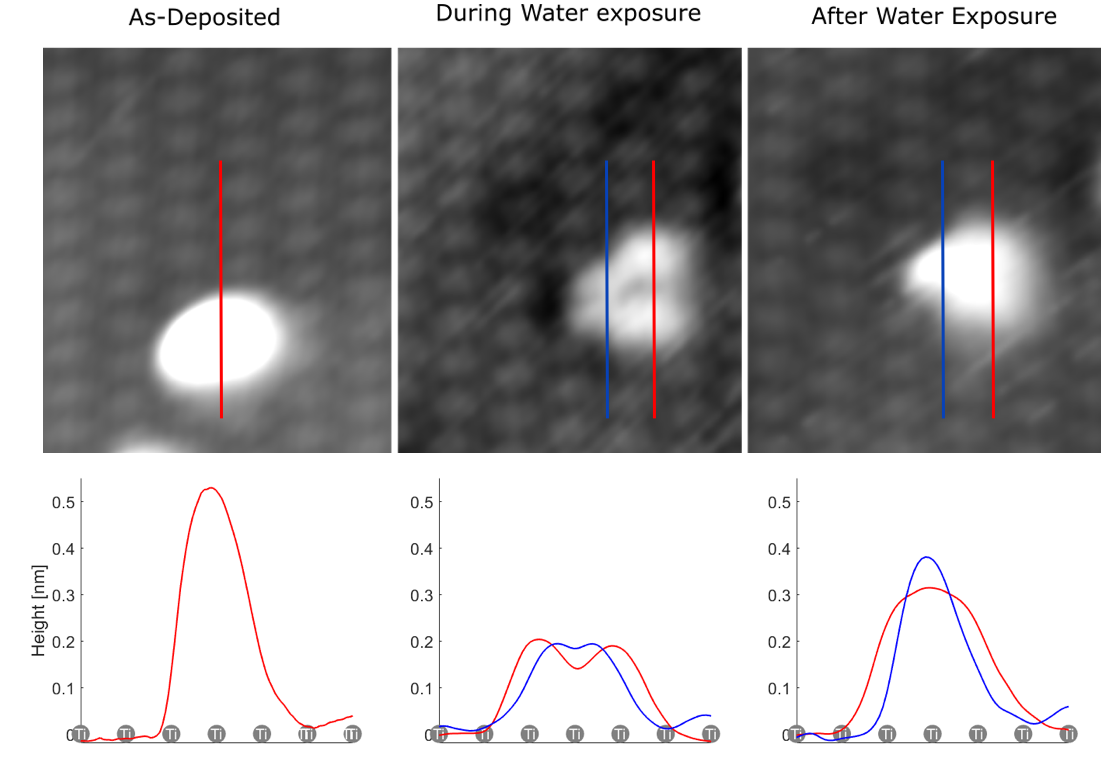
\includegraphics[width=1.0\textwidth]{Expert_claim.png}
\caption{Experimental Observation}
\label{fig:exptobser}
\end{figure*}

\section{Fundamental questions raised from theory}
$i)$ There is no clear evidence that what is the molecular form of these features
$ii)$  Why same features were not observed after and during water exposure 
$iii)$ No clear evidence of what is the composition of oxygen while formation of oxide clusters 

\section{Methodology}

\begin{figure*}
\centering
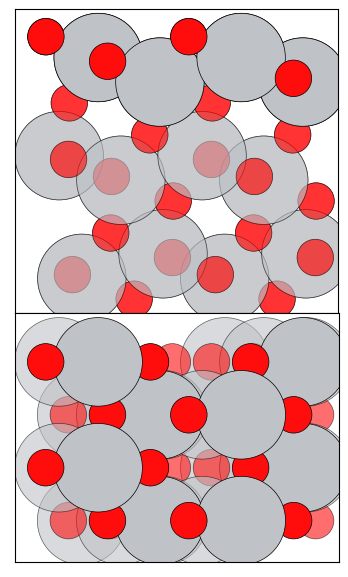
\includegraphics[width=0.2\textwidth]{TiO2_101sur_2by1supercell.png}
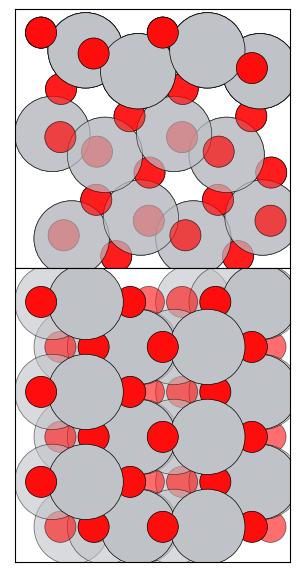
\includegraphics[width=0.2\textwidth]{TiO2_101sur_3by1supercell.png}
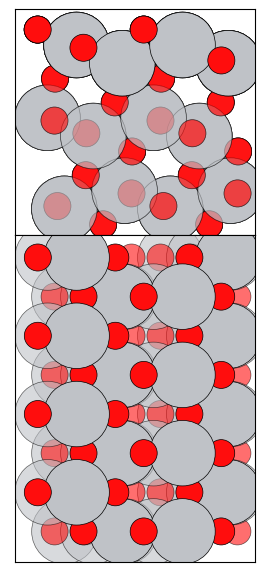
\includegraphics[width=0.2\textwidth]{TiO2_101sur_4by1supercell.png}
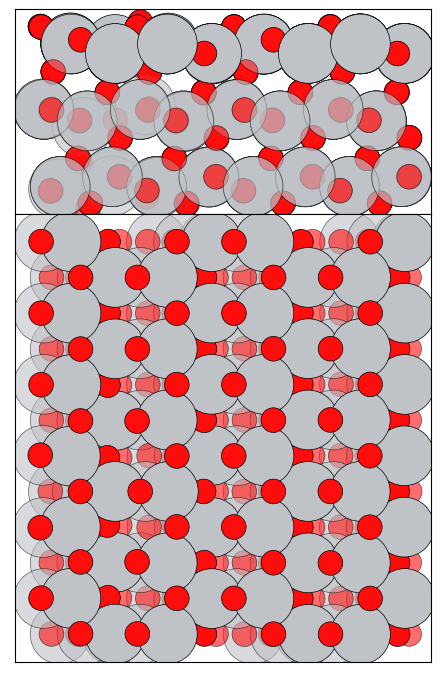
\includegraphics[width=0.4\textwidth]{TiO2_101sur_6by2supercell.png}
\caption{Different super cell size of surfaces used in all the calculations.}
\label{fig:exptobser}
\end{figure*}
\section{Results}
\subsection{low-lying isomers found for VO$_2$ , VO$_2$H$_2$O and VO$_2$2H$_2$O clusters}
\begin{figure*}
\centering
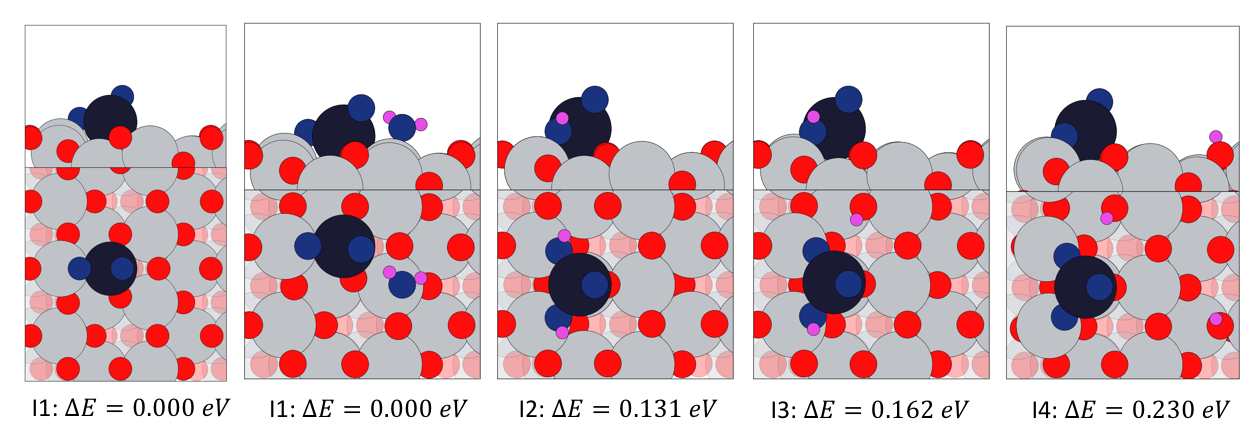
\includegraphics[width=1.0\textwidth]{VO2_VO2H2Oclusters_TiO2_101sur_2by1supercell.png}
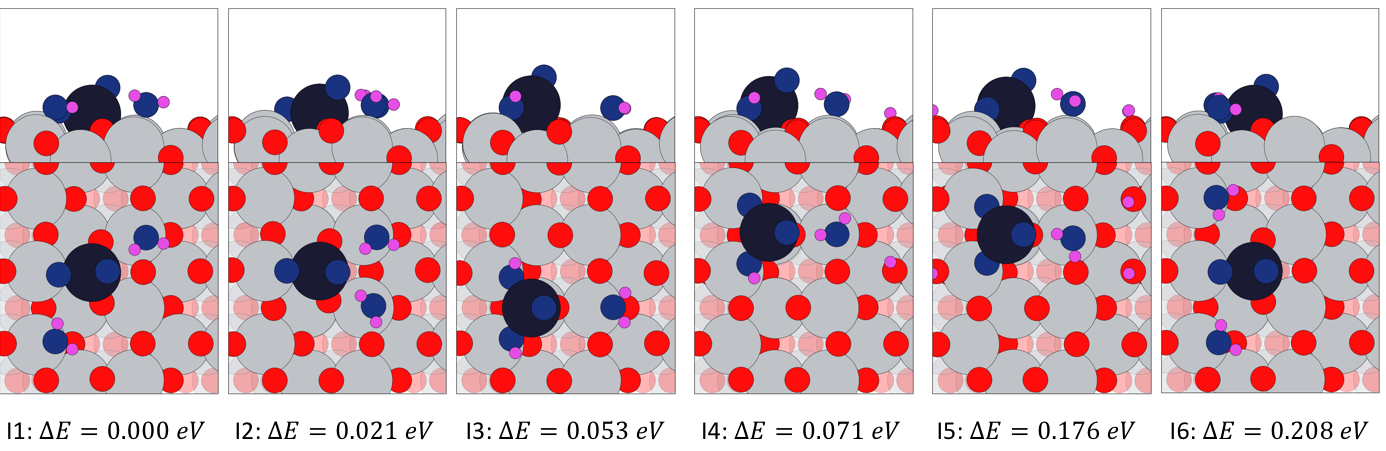
\includegraphics[width=1.0\textwidth]{VO2_2H2Oclusters_TiO2_101sur_3by1supercell.png}
\caption{All the possible low-lying isomers found for VO$_2$ , VO$_2$H$_2$O and VO$_2$2H$_2$O clusters with GOFEE were DFT relaxed with one Oxygen vacancy created in 2nd layer. Here two types of super cell sizes were used those are $2 \times 1 \times 1$ super cell for VO$_2$ , VO$_2$H$_2$O and  $3 \times 1 \times 1$ super cell for VO$_2$2H$_2$O clusters.}
\label{fig:exptobser}
\end{figure*}

\subsection{low-lying isomers found for V$_2$O$_4$ , V$_2$O$_4$H$_2$O and V$_2$O$_4$2H$_2$O clusters}

\begin{figure*}
\centering
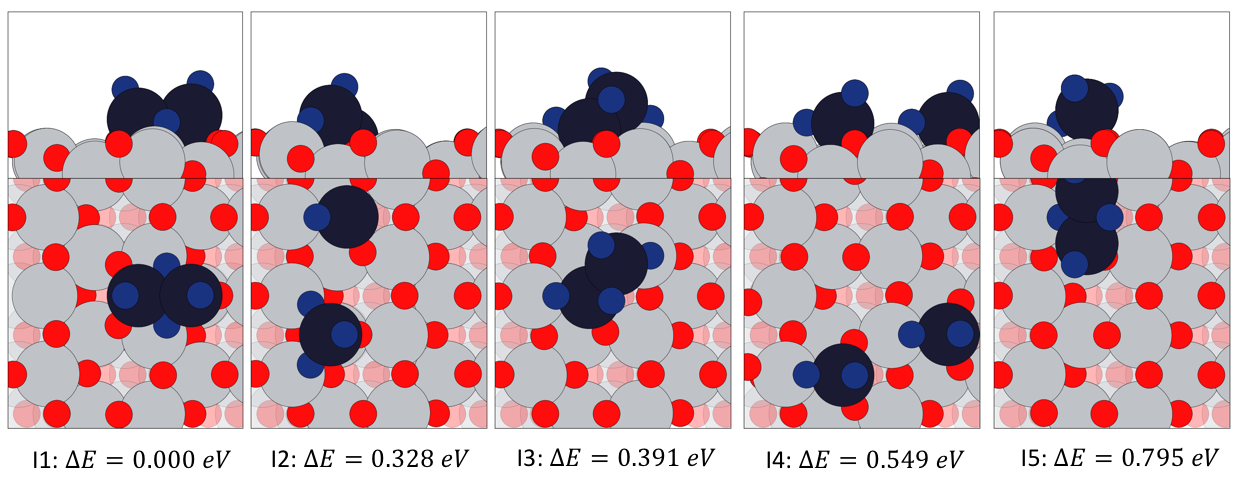
\includegraphics[width=1.0\textwidth]{V2O4_TiO2_101sur_3by1supercell.png}
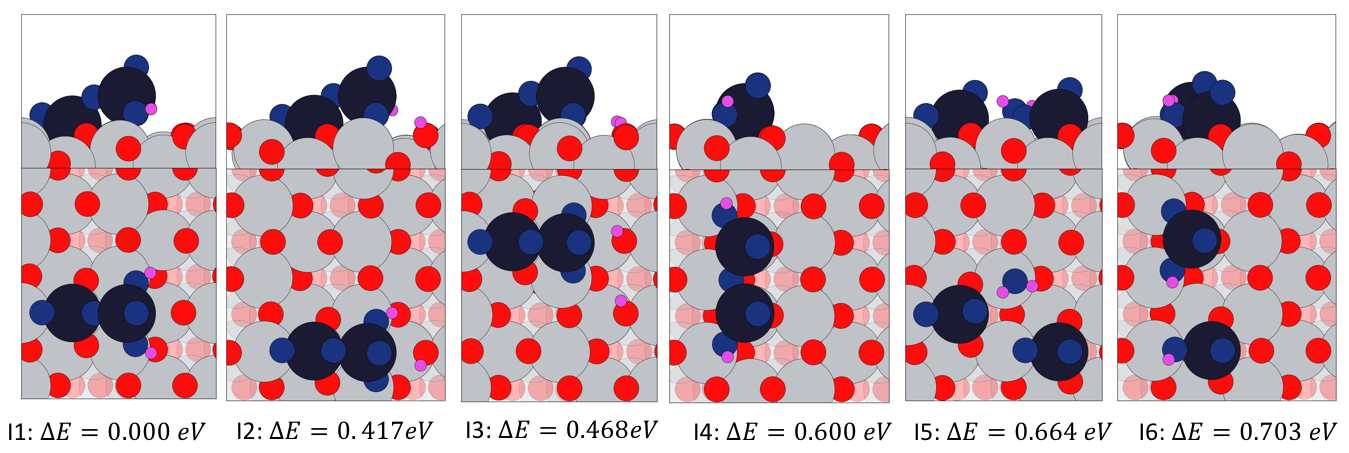
\includegraphics[width=1.0\textwidth]{V2O4_H2O_TiO2_101sur_3by1supercell.png}
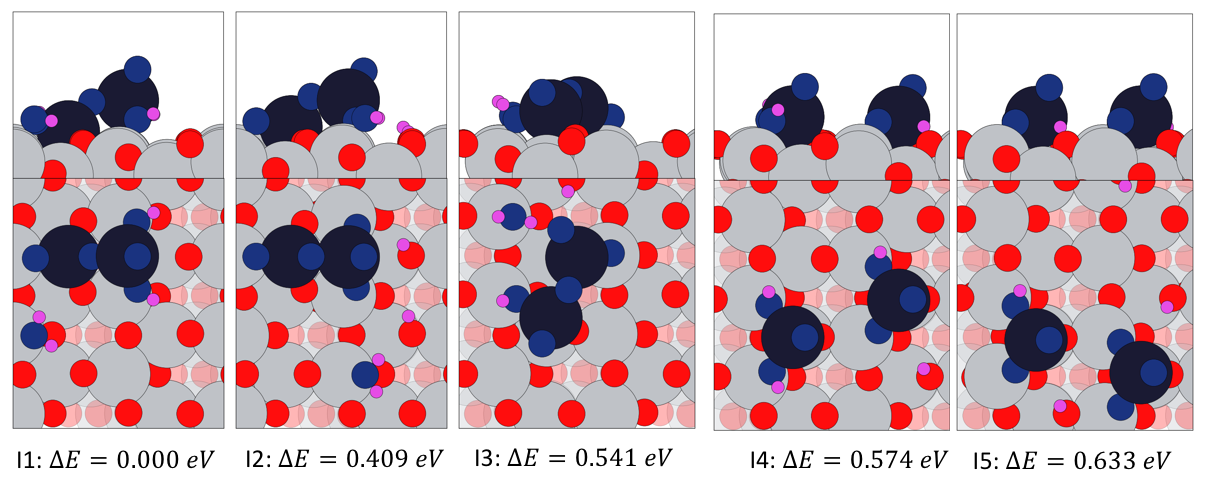
\includegraphics[width=1.0\textwidth]{V2O4_2H2O_TiO2_101sur_3by1supercell.png}
\caption{All the possible low-lying isomers found for V$_2$O$_4$  , V$_2$O$_4$ H$_2$O and V$_2$O$_4$ 2H$_2$O clusters with GOFEE were DFT relaxed with one Oxygen vacancy created in 2nd layer. Here $3 \times 1 \times 1$ super cell used for all clusters.}
\label{fig:exptobser}
\end{figure*}

\subsection{low-lying isomers found for V$_2$O$_5$ , V$_2$O$_5$H$_2$O and V$_2$O$_5$2H$_2$O clusters}

\begin{figure*}
\centering
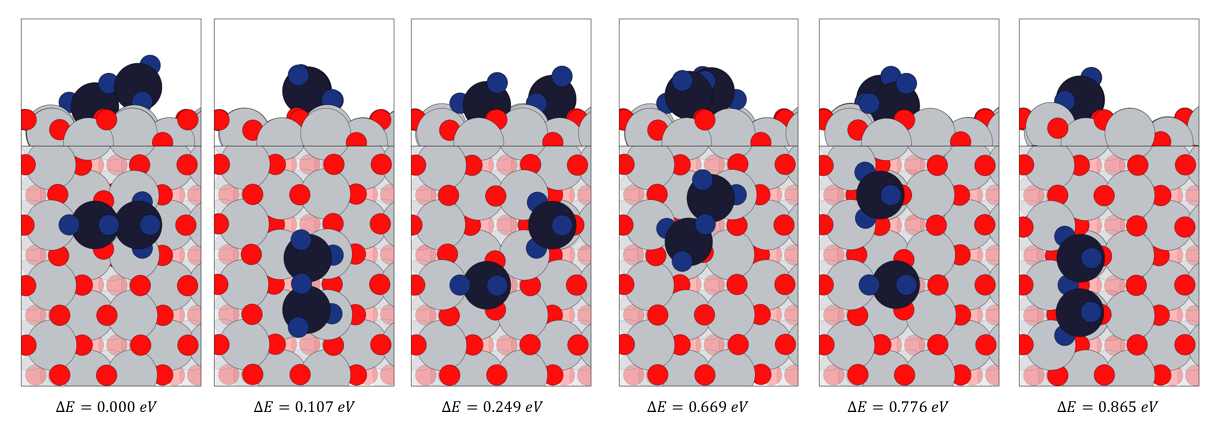
\includegraphics[width=1.0\textwidth]{V2O5_TiO2_101sur_4by1supercell.png}
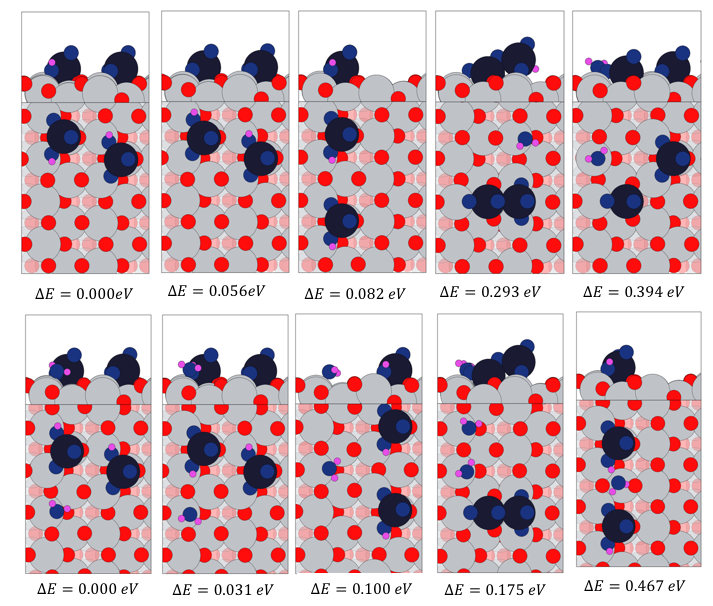
\includegraphics[width=1.0\textwidth]{V2O5_2H2O_H2O_TiO2_101sur_4by1supercell.png}
\caption{All the possible low-lying isomers found for V$_2$O$_5$  , V$_2$O$_5$H$_2$O and V$_2$O$_5$2H$_2$O clusters with GOFEE were DFT relaxed with one Oxygen vacancy created in 2nd layer. Here $4 \times 1 \times 1$ super cell used for all clusters.}
\label{fig:exptobser}
\end{figure*}

\subsection{Binding Energies for V$_2$O$_5$ , V$_2$O$_5$H$_2$O and  V$_2$O$_5$2H$_2$O clusters}
\begin{figure*}
\centering
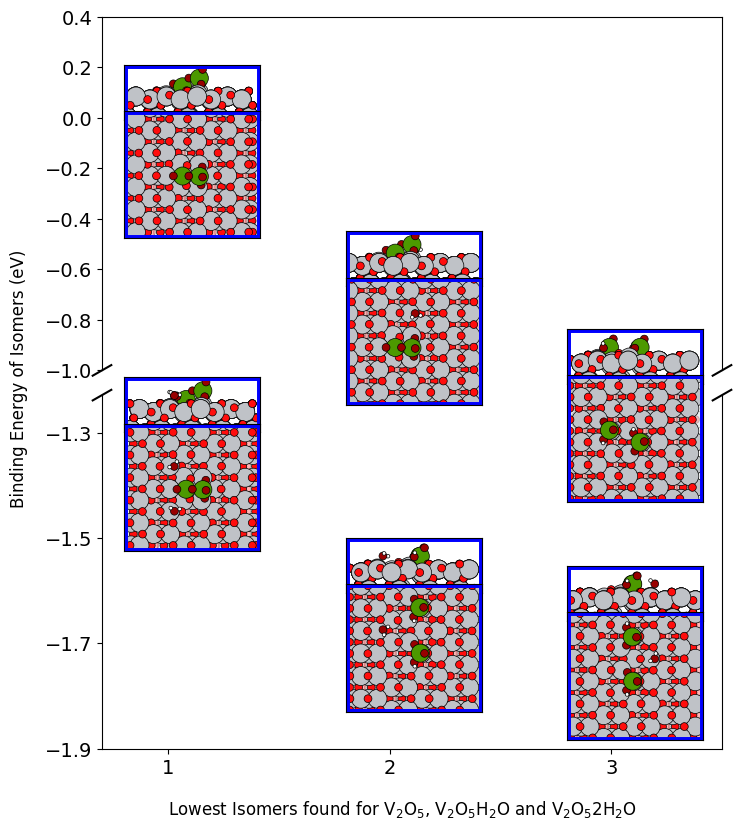
\includegraphics[width=1.0\textwidth]{BE_order_1Ov_2ndrow_V2O5clu_TiO2_101sur.png}
\caption{Binding energy order for best structures of V$_2$O$_5$ , V$_2$O$_5$ H$_2$O and V$_2$O$_5$ 2H$_2$O clusters found in global optimization were re-optimised with $6 \times 2 \times 1$ super cell  and  one oxygen vacancy created.}
\label{fig:BE_1Ov}
\end{figure*}
%--------------------------------------------------------%
\begin{figure*}
\centering
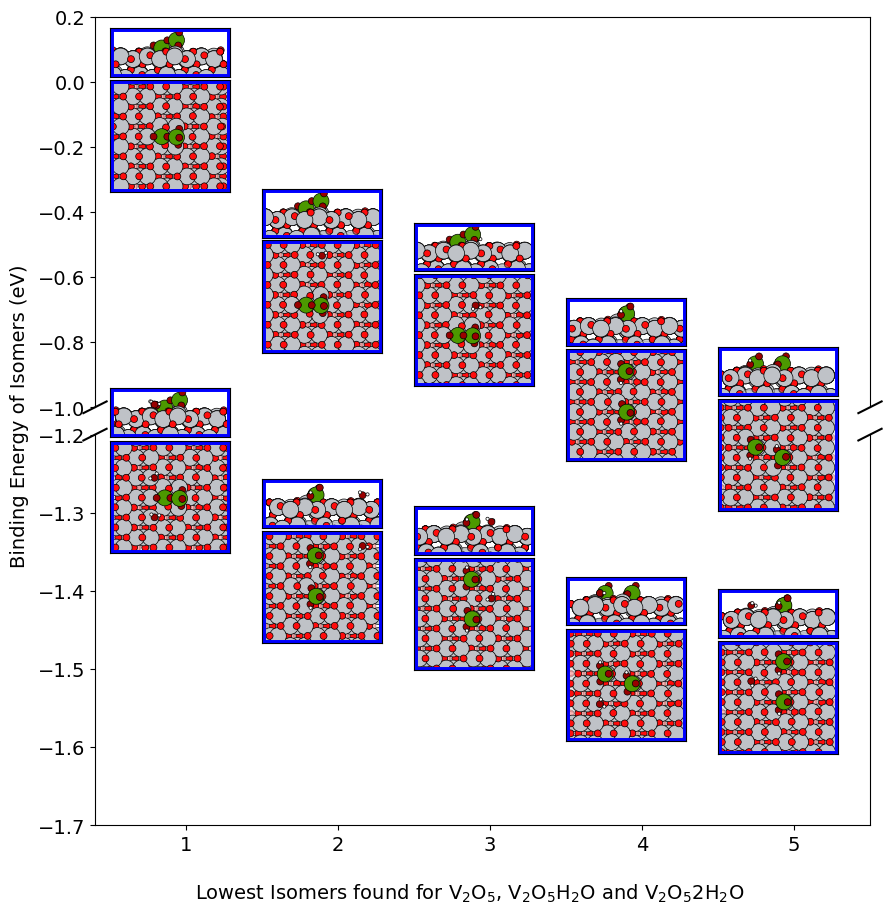
\includegraphics[width=1.0\textwidth]{BE_order_2Ov_V2O5clu_TiO2_101sur.png}
\caption{Binding energy order for best structures of V$_2$O$_5$ , V$_2$O$_5$ H$_2$O and V$_2$O$_5$ 2H$_2$O clusters found in global optimization were re-optimised with $6 \times 2 \times 1$ super cell  and  two oxygen vacancy created.}
\label{fig:BE_1Ov}
\end{figure*}
\section{NEB calculation on $4\times 1$ cell for VO$_3$H diffusion}
\begin{figure*}
\centering
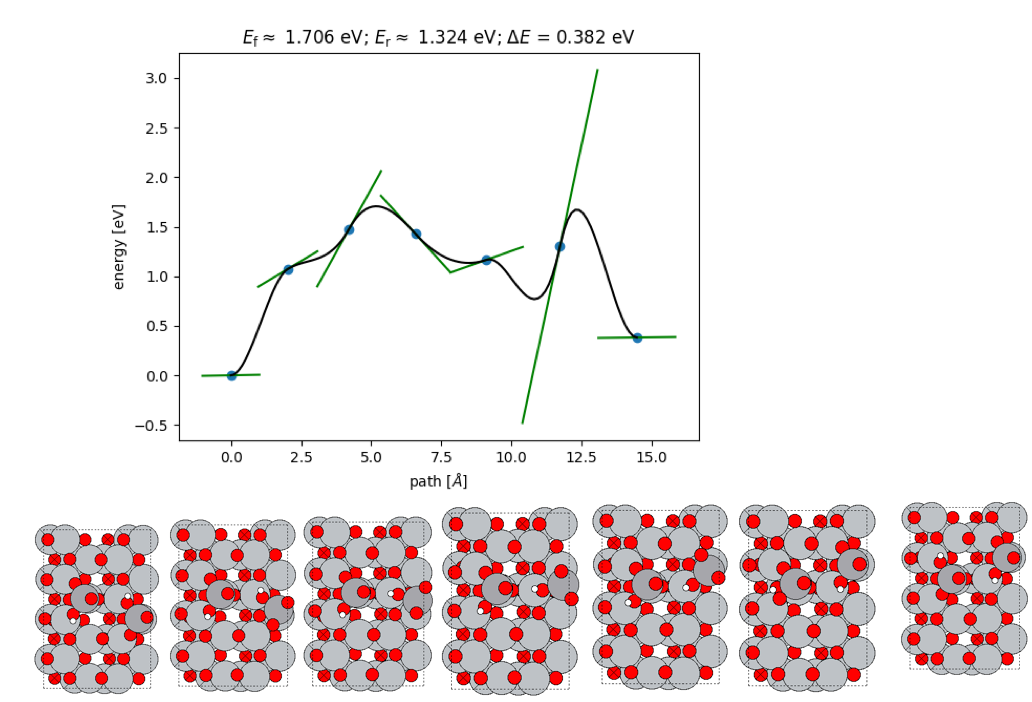
\includegraphics[width=1.0\textwidth]{NEB_calculation_4by1cell_2VO3Hdiffusion.png}
\caption{NEB calculations}
\label{fig:BE_1Ov}
\end{figure*}
\section{References}
\bibliography{bib}

\end{document}


